\documentclass[tikz,border=10pt]{standalone}
\usepackage{tikz}
\usetikzlibrary{arrows.meta}

\begin{document}
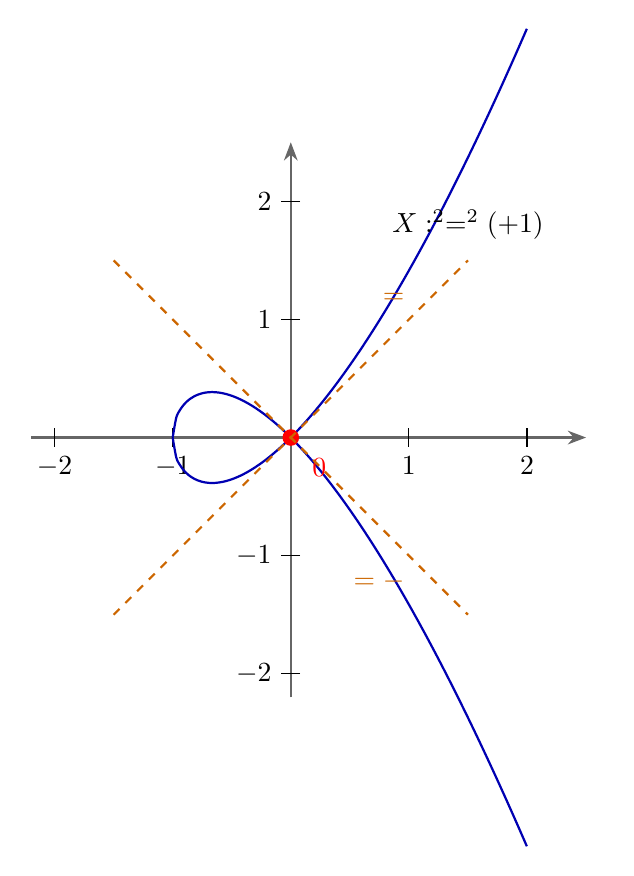
\begin{tikzpicture}[
    scale=1.5,
    >=Stealth,
    axis/.style={->,thick,black!60},
    curve/.style={thick,blue!70!black,smooth}
]
    % Axes
    \draw[axis] (-2.2,0) -- (2.5,0) node[right] {$\x$};
    \draw[axis] (0,-2.2) -- (0,2.5) node[above] {$\y$};
    
    % Tick marks
    \foreach \x in {-2,-1,1,2} {
        \draw (\x,0.08) -- (\x,-0.08) node[below] {$\x$};
    }
    \foreach \y in {-2,-1,1,2} {
        \draw (0.08,\y) -- (-0.08,\y) node[left] {$\y$};
    }
    
    % Node curve: y^2 = x^2(x+1), so y = ±x*sqrt(x+1)
    % Domain: x >= -1
    \draw[curve,domain=-1:2,samples=100,variable=\x] 
        plot ({\x},{\x*sqrt(\x+1)});
    \draw[curve,domain=-1:2,samples=100,variable=\x] 
        plot ({\x},{-\x*sqrt(\x+1)});
    
    % Origin (singular point)
    \fill[red] (0,0) circle (2pt);
    \node[red,below right] at (0.1,-0.1) {$0$};
    
    % Tangent lines at origin (dashed)
    \draw[dashed,orange!80!black,thick] (-1.5,-1.5) -- (1.5,1.5) 
        node[pos=0.85,above left] {$\y=\x$};
    \draw[dashed,orange!80!black,thick] (-1.5,1.5) -- (1.5,-1.5) 
        node[pos=0.85,below left] {$\y=-\x$};
    
    % Label
    \node at (1.5,1.8) {$X: \y^2 = \x^2(\x+1)$};
    
\end{tikzpicture}
\end{document}
